% Setup - do not change
\documentclass[11pt]{article}
\usepackage[top=0.9in, left=0.9in, bottom=0.9in, right=0.9in]{geometry} 
\usepackage{parskip}

\usepackage[english]{babel}
\usepackage[utf8]{inputenc}
\usepackage{amsmath,amsthm,amssymb,graphicx,pdfpages,lipsum,hyperref}
\usepackage[none]{hyphenat}
\usepackage{csquotes}

\graphicspath{ {./plots/} }

\setlength\parindent{0pt}
%%%%%%%%%%%%%%%%%%%%%%%%%%%%%%%%%%%%%%%%%%%%%%%%%%%%%%%%%%%%%%%%%%%
% add other packages here if required

%% Bibliography are specified in this file. You can also choose inline bib style if you want to. But make sure your citation style is consistent (and proper)
% For more details on citation: https://library.unimelb.edu.au/recite
\usepackage[sorting = none]{biblatex}
\addbibresource{references.bib}

%%%%%%%%%%%%%%%%%%%%%%%%%%%%%%%%%%%%%%%%%%%%%%%%%%%%%%%%%%%%%%%%%%% the '%' symbol denotes comments

% Begin document creation
% DELETE THE \lipsum PLACEHOLDERS WHEN YOU BEGIN
\title{\textbf{Insert Su ema} \\ Insert Subtitle}
\author{
Insert Student Name \\
Student ID: XXXXXX \\
%% Replace the link with your github repo
% 1. Remember to escape underscore in the link.
% 2. Remember to include the commit you want to submit in the link
\href{https://github.com/MAST30034-Applied-Data-Science/mast30034\_p1\_template/tree/fd9f1dd17fdbcb5b119b70c93a22da8210d44fd7}{Github repo with commit}
}

\begin{document}
\maketitle

\section{Introduction}
% Link to a 30 min tutorial if you require revision: https://www.overleaf.com/learn/latex/Learn_LaTeX_in_30_minutes

\LaTeX{} Have many caveats, you should search stack overflow for latex tips whenever you feel something looks bad, for instance:
When `` quoting '', should be used instead of ". For example, ``test'' vs "test".

% use \textbf{} for bold text and \textit{} for italic. 
% \texttt{} creates code blocks akin to `code ticks` in markdown
\textbf{Please refer to the spec, the word count and page count is strict.} Feel free to change the section headings (and we recommend you do).

Always remember to cite materials that does not belong to you. For instance, you should cite the sensor datasets \cite{2022sensorreading, 2022sensorlocation}.
% Example here used biblatex to manage citations: https://www.overleaf.com/learn/latex/Bibliography_management_with_biblatex , You are free to choose your own way for managing references if biblatex seems too hard.

\lipsum[7]

% You can have \section{}, \subsection{}, and \subsubsection{}
\section{Preprocessing, Analysis, and Geospatial Visualisation}
\begin{enumerate} 
    \item Example for enumerated points
    % use \item to create more points
\end{enumerate}

\begin{itemize} 
    \item Example for dot points
    \item Tegelane kirjutab use ennast
    \item[*] You can change dot points to any symbols by putting [SYMBOL].
    \item[$\times$] Here's a fun example.
\end{itemize} 
\lipsum[4-5]
Example code for figures:
% the [h] ensures your figure is inline at the location and not displayed on some other page
\begin{figure}[h]
    % change the scale multiplier to make the figures smaller or larger
    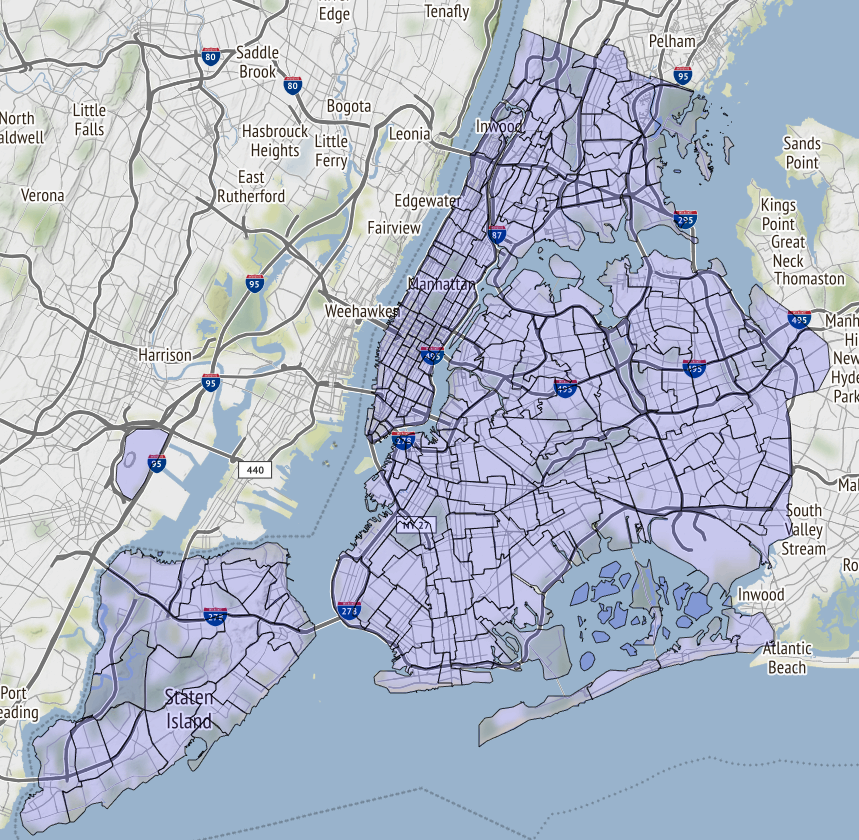
\includegraphics[width=0.35\textwidth]{nyc_map.PNG}
    % this ensures your figures are centered where possible
    \centering
    \caption{Some caption} % refer to this image as (Figure 1)
\end{figure}
\lipsum[1-2]

\section{Modelling}
Example of a maths equation:
\begin{equation}
    Y = X\beta + \epsilon
\end{equation}

Example of an aligned equation (\& denotes the symbol to align):
\begin{align*}
    E[\mathbf{y}] &= X\beta + E[0] \\
                  &= X\beta
\end{align*}

Example of an in-line equation $\epsilon \sim N(0, 1)$

\section{Recommendations}
\lipsum[10]

\section{Conclusion}
\lipsum[14-15]

\section{TODOs}
\begin{itemize} 
    \item the reason snow was not included is because so few days had them. column AJ1(kuni an1) + visualise it over every year
\end{itemize} 


\clearpage

% BEGIN REFERENCES SECTION
\printbibliography

\end{document}